\section{Unit test Naiad Power-board 4.4}
\label{Unit_PSU}
\label{A_powerboard}
This is a unit test for The Naiad power-board 4.4. This guide can also be used to understand the different parts of the power board. It covers most of the power board but does not go in to detail to check the temperature and voltage monitoring featured on the card. 
\subsection {Required resources}
\begin{itemize}
\item Power board to test
\item Power supply, 22-24V
\item Multi-meter
\item Working CAN-card with software that sets digital 3,4 high and control PWM 1, 2, 3 as well as take input on digital 7.
\end{itemize}

\newpage
\subsection{Input and prio-electronics}
Plug in the card in at least one of the four supply terminal block located in the bottom of the card to a suitable source. 22-24V with minimum of 500 mA for testing is sufficient. \textbf{The ground is always the lead \emph{closest} to the fuse!} You need to flip the cables if plugged on to Ext1 or Ext2 according to figure ref{input}.


\begin{figure}[!ht]
	\begin{center}
		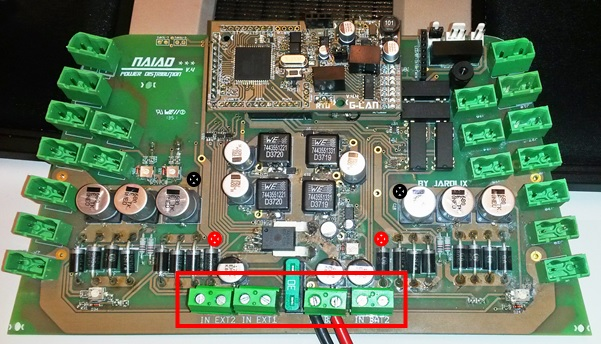
\includegraphics[width=0.76\textwidth]{./Images/Unit_test_power_board/Input.jpg}
		\caption{The caption you want with the picture}
		\label{input}
	\end{center}
\end{figure}

\begin{table}[ht]
\begin{tabularx}{\textwidth}{|c|>{\hsize=0.6\hsize}X|>{\hsize=0.6\hsize}X|c|>{\hsize=1.8\hsize}X|} %>{\hsize=.5\hsize}X>
\hline 
Point/Net & Precondition: & Desired & Measured & Commentary \\ 
\hline 
GND & Supply with 22-24 V and 500 mA & 0V / 0$\Omega$ &   & Make sure the black dots and the ground on the supply are connected. If not, discard the card.  \\ 
\hline 
Input & Supply with 22-24 V and 500 mA & Input voltage 22-24V &    & Make sure the That the voltage is correct and then that the wires are in the correct socket on the terminal block. If all these are correct check the Fuse.   \\ 
\hline 
Fuse & - & 30 A Car fuse &   & Try another Fuse. If still no power is supplied to rest of card check the two points marked.  \\ 
\hline 
Prio-volt & Supply with 22-24 V and 500 mA & Input voltage 22-24V &    & If there still is no power on the dots there is either a problem with the terminal blocks or the diodes next to the dots. Change these and try again. If there is power here but the CAN-card is not lit, check the trace leading to the CAN-card power supply for damage.  \\ 
\hline
\end{tabularx}
\end{table}

\newpage
\subsection{Required peripherals on PSU}
\begin{figure}[!ht]
	\begin{center}
		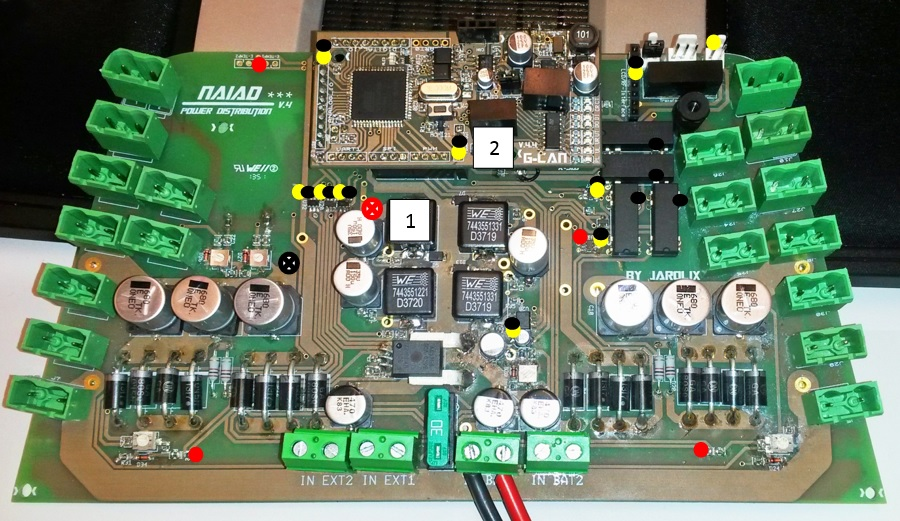
\includegraphics[width=0.7\textwidth]{./Images/Unit_test_power_board/peripherals.jpg}
		%\caption{The caption you want with the picture}
		\label{peripherals}
	\end{center}
\end{figure}

\begin{table}[ht]
\begin{tabularx}{\textwidth}{|c|>{\hsize=0.6\hsize}X|>{\hsize=0.6\hsize}X|c|>{\hsize=1.8\hsize}X|} 
\hline 
Point/Net & Precondition: & Desired & Measured & Commentary \\ 
\hline 
Const 5V & Supply and Prio-volt works. & 5V &   & This is used at several point on the card, but firstly check that the output is correct from the DC-DC regulator by measuring on point text to the box with a 1 in it.  \\ 
\hline
Const 5V & Supply and Prio-volt works. & 5V &   & Check the rest of the points smaller points, all should be 5V compared to the larger black it the above point but not one of these points a trace is broken.  \\ 
\hline
MCU\_VCC & Working CAN-card & 5V &   & Firstly make sure that the CAN-card is working, then measure on the CAN-card between VCC out and GND, the small yellow and black next to the 2.  \\ 
\hline 
MCU\_VCC & Working CAN-card & 5V &   & Measure between all small black points and small yellow points, all should be 5V if the MCU VCC in 5V but not one of these points a trace is broken. (On the IC on the left it is the left most legs that should be measured, there is also another on the underside below the E-temp connector\' s).  \\ 
\hline
\end{tabularx}
\end{table}

\newpage
\subsection{Kill switch / Mission switch}
The mission switch sets digital pin 1 high.
\begin{figure}[!ht]
	\begin{center}
		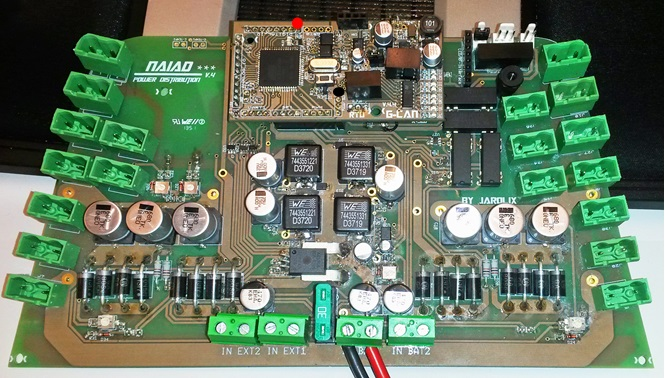
\includegraphics[width=0.76\textwidth]{./Images/Unit_test_power_board/kill_mission.jpg}
		%\caption{The caption you want with the picture}
		\label{motor_pwr}
	\end{center}
\end{figure}

\begin{table}[ht]
\begin{tabularx}{\textwidth}{|>{\hsize=0.6\hsize}X|>{\hsize=0.8\hsize}X|>{\hsize=0.8\hsize}X|c|>{\hsize=1.8\hsize}X|}
\hline
Point/Net & Precondition: & Desired & Measured & Commentary \\ 
\hline
Mission switch & Working CAN-card & 5V &   & Short the two pins on the mission switch. Then digital 1 should be 5V compared to MCU GND(the small red and black dot) \\ 
\hline 
Kill switch & Supply with 22-24 V &  &  & When the pins are NOT shorted a red LED under the CAN-card should be lit. When the two connectors are connected the red light goes out. CAN-power is still on when the kill switch is disconnected but the motor power should be killed. Check these by measuring the CAN and motor output. \\ 
\hline 
\end{tabularx}
\end{table}

\newpage
\subsection{Can-Power}
\begin{figure}[!ht]
	\begin{center}
		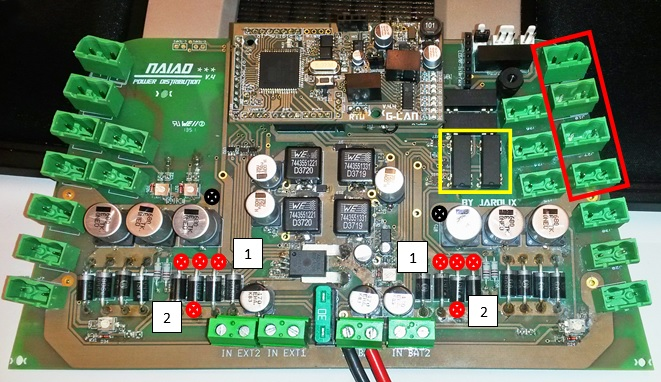
\includegraphics[width=0.76\textwidth]{./Images/Unit_test_power_board/can_pwr.jpg}
		%\caption{The caption you want with the picture}
		\label{can_pwr}
	\end{center}
\end{figure}

\begin{table}[ht]
\begin{tabularx}{\textwidth}{|>{\hsize=0.6\hsize}X|>{\hsize=0.8\hsize}X|>{\hsize=0.8\hsize}X|c|>{\hsize=1.8\hsize}X|}
\hline 
 Point/Net & Precondition: & Desired & Measured & Commentary \\ 
\hline
Output & Software that enables Electronics & Input voltage
22-24V &   & Make sure it seems like the terminal blocks have contact with the trace. If they do try the points marked in the picture next to the 1  \\ 
\hline 
Can-power (dots 1) & Supply with 22-24 V and 500 mA & Input voltage 22-24V &    & If there is power here but not in the terminal block there is some kind of damage on the trace between this point and the output. \\ 
\hline 
Can-power (dots 2) & - & Input voltage 22-24V &   & If there is power here but not at (1) there is something wrong with the Diode, change the diodes and try again. If not turn the card over and measure the switches. \\ 
\hline 
Switch (marked yellow) &  & 0$\Omega$(or close)&    & The second leg need to be shorted to GND via a relay controlled by PWM 3. If it is not make sure the software is working and that the traces are undamaged. Try to ground the second leg or change the switches \\ 
\hline
\end{tabularx}
\end{table}

\newpage
\subsection{Motor power}
The power for the motors can be taken from the bottom three connectors on both sides of the card, these have to be activated in the software by setting digital 3 to high on the CAN-card.
\begin{figure}[!ht]
	\begin{center}
		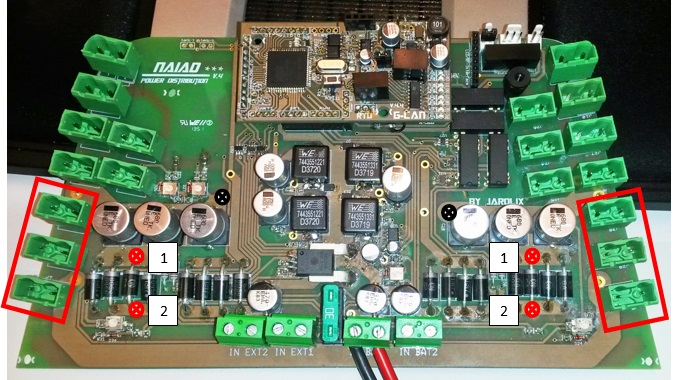
\includegraphics[width=0.76\textwidth]{./Images/Unit_test_power_board/motor_pwr.jpg}
		%\caption{The caption you want with the picture}
		\label{motor_pwr}
	\end{center}
\end{figure}

\begin{table}[ht]
\begin{tabularx}{\textwidth}{|>{\hsize=0.6\hsize}X|>{\hsize=0.8\hsize}X|>{\hsize=0.8\hsize}X|c|>{\hsize=1.8\hsize}X|}
\hline 
 Point/Net & Precondition: & Desired & Measured & Commentary \\ 
\hline
Kill switch &  &  &  & Make sure that the kill-switch's two pins are connected, the kill switch light should go out. \\ 
\hline
Output & Software that enables motors & Input voltage 22-24V &   & Make sure it seems like the terminal blocks have contact with the trace. If they do try the points marked in the picture next to the 1. \\ 
\hline 
Motor Power (dots 1) & Supply with 22-24 V and 500 mA & Input voltage 22-24V &    & If there is power here but not in the terminal block there is some kind of damage on the trace between this point and the output. \\ 
\hline 
Motor Power (dots 2) & Supply with 22-24 V and 500 mA  & Input voltage 22-24V &   & If there is power here but not at (1) there is something wrong with the Diode, change the diodes and try again. 
If not turn the card over and measure the switches on the back \\ 
\hline 
\end{tabularx}
\end{table}

\newpage
\subsection{Headlight}
These outputs are in the Ultiboard and Multisim file called Headlight but they are really a adjustable output voltage between 1.8 to 22V, all of the connectors have the same voltage however. They use the CAN-power which therefore need to work and be activated. To control these a digital potentiometer is changed by triggering pin PWM1 and PWM2. PWM1 decreases the voltage and the PWM2 increases one step for each pulse. 
\begin{figure}[!ht]
	\begin{center}
		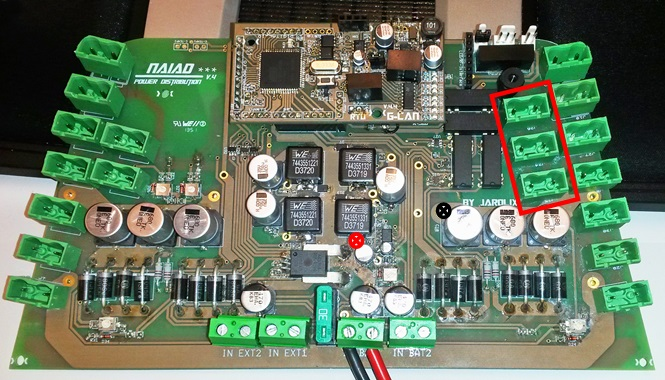
\includegraphics[width=0.76\textwidth]{./Images/Unit_test_power_board/headlight.jpg}
		%\caption{The caption you want with the picture}
		\label{motor_pwr}
	\end{center}
\end{figure}

\begin{table}[ht]
\begin{tabularx}{\textwidth}{|>{\hsize=0.6\hsize}X|>{\hsize=0.8\hsize}X|>{\hsize=0.8\hsize}X|c|>{\hsize=1.8\hsize}X|}
\hline
Point/Net & Precondition: & Desired & Measured & Commentary \\ 
\hline
Output & CAN-power working, Working MCU GND and MCU VCC & Input voltage 22-24V &   & Make sure it seems like the terminal blocks have contact with the trace. If they do try the point marked in the picture. \\ 
\hline 
Headlight Power(dots) &  & Input voltage 22-24V &    & If there is power here but not in the terminal block there is some kind of damage on the trace between this point and the output. If not check DC-DC on the underside. \\ 
\hline 
DC-DC &  & 	1:output voltage 2:22-24V 3:22-24V 4:0V 5:NaN 6:unkown 7:5V &   & If these are not correct check with the schematic for possible solution.  \\ 
\hline 
\end{tabularx}
\end{table}

\newpage
\subsection{12 V}
12 V output (however are more close to 11.6) are enabled together with motors and requires CAN-power to function. 
\begin{figure}[!ht]
	\begin{center}
		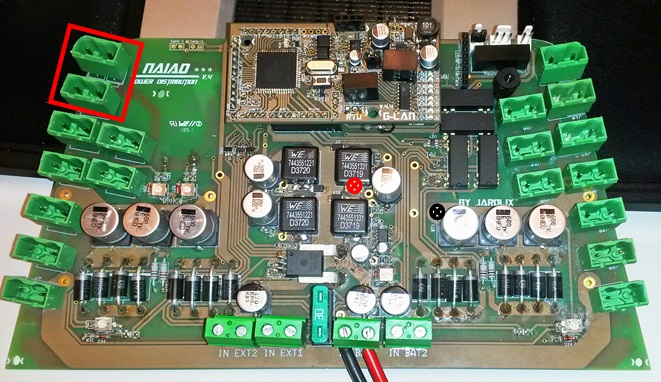
\includegraphics[width=0.76\textwidth]{./Images/Unit_test_power_board/12v.jpg}
		%\caption{The caption you want with the picture}
		\label{motor_pwr}
	\end{center}
\end{figure}

\begin{table}[ht]
\begin{tabularx}{\textwidth}{|>{\hsize=0.6\hsize}X|>{\hsize=0.8\hsize}X|>{\hsize=0.8\hsize}X|c|>{\hsize=1.8\hsize}X|}
\hline
Point/Net & Precondition: & Desired & Measured & Commentary \\ 
\hline
Output & Can-power working and kill-switch activated. & 12V &   & Make sure it seems like the terminal blocks have contact with the trace. If they do try the point marked in the picture. \\ 
\hline 
12V (dots) &  & Input voltage 22-24V &    & If there is power here but not in the terminal block there is some kind of damage on the trace between this point and the output. If not check DC-DC on the underside. \\ 
\hline 
DC-DC &  & 	1:12V 2:22-24V 3:22-24V 4:0V 5:NaN 6:unkown 7:5V &   & If these are not correct check with the schematic for possible solution.  \\ 
\hline 
\end{tabularx}
\end{table}

\newpage

\newpage
\subsection{5 V}
5V output are enabled by setting digital 4 high and requires CAN-power. 
\begin{figure}[!ht]
	\begin{center}
		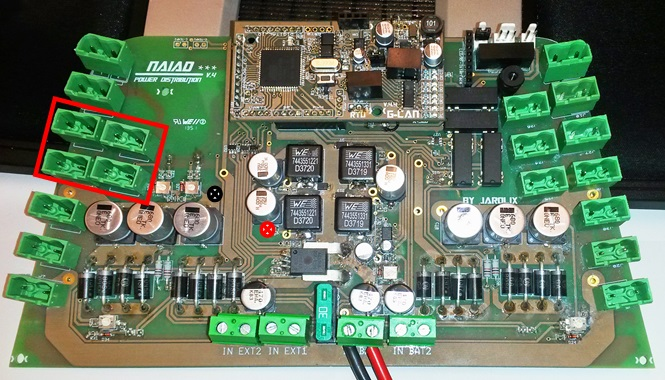
\includegraphics[width=0.76\textwidth]{./Images/Unit_test_power_board/5v.jpg}
		%\caption{The caption you want with the picture}
		\label{motor_pwr}
	\end{center}
\end{figure}

\begin{table}[ht]
\begin{tabularx}{\textwidth}{|>{\hsize=0.6\hsize}X|>{\hsize=0.8\hsize}X|>{\hsize=0.8\hsize}X|c|>{\hsize=1.8\hsize}X|}
\hline
Point/Net & Precondition: & Desired & Measured & Commentary \\ 
\hline
Output & CAN-power working software that enables electronics (Digital pin 4 and PWM 3) & 5V &   & Make sure it seems like the terminal blocks have contact with the trace. If they do try the point marked in the picture. \\ 
\hline 
5V (dots) &  & Input voltage 22-24V &    & If there is power here but not in the terminal block there is some kind of damage on the trace between this point and the output. If not check DC-DC on the underside. \\ 
\hline 
DC-DC &  & 	1:5V 2:22-24V 3:22-24V 4:0V 5:NaN 6:unkown 7:5V &   & If these are not correct check with the schematic for possible solution.  \\ 
\hline 
\end{tabularx}
\end{table}

\newpage